\section{Resultados}
\label{sec:resultados}

\subsection{RQ01--RQ04: métricas e referência C1}

A Tabela~\ref{tab:metricas-final} reúne as variantes. O CFR~(b) tem
\labACfrBN\ observações e a recuperação, \labARecN; as ausências não são imputadas.

\begin{table}[htbp]
\centering\footnotesize
\caption{Medianas e quartis; peso igual por projeto, exceto episódios na última linha.}
\label{tab:metricas-final}
% Gerado por analises.sprint3_a; não edite à mão.
\begin{tabular}{lllrrrr}
\hline
RQ & Métrica & Unidade & $n$ & Mediana & Q1--Q3 & IQR \\
\hline
RQ01 & Frequência: releases & por semana & 300 & 0,326 & 0,153--0,825 & 0,671 \\
RQ01 & Frequência: com pré-releases & por semana & 300 & 0,345 & 0,173--0,863 & 0,690 \\
RQ01 & Frequência: tags & por semana & 300 & 0,403 & 0,192--1,016 & 0,825 \\
\hline
RQ02 & Lead time (a): por release & horas & 300 & 196,7 & 47,26--715,6 & 668,3 \\
RQ02 & Lead time (b): por commit & horas & 300 & 178,3 & 43,10--475,4 & 432,3 \\
\hline
RQ03 & CFR (a): runs de CI & proporção & 300 & 0,055 & 0,024--0,129 & 0,105 \\
RQ03 & CFR (b): releases & proporção & 289 & 0,175 & 0,000--0,429 & 0,429 \\
\hline
RQ04 & Recuperação: mediana por projeto & horas & 278 & 3,20 & 0,60--18,37 & 17,77 \\
RQ04 & Recuperação: episódios concluídos & horas & 7.771 & 3,57 & 0,88--20,28 & 19,40 \\
\hline
\end{tabular}

\end{table}

\textbf{RQ01.} A frequência mediana de \labAFreqMediana\ release/semana equivale
a aproximadamente uma a cada três semanas. Só \labAFreqSemanais\ projetos
(\labAFreqSemanaisPct\%) chegam a uma por semana e \labAFreqDiarios\ a sete.
Incluir pré-releases eleva a mediana a \labAFreqPreMediana; tags, a
\labAFreqTagsMediana. A cauda à direita e a baixa mediana sustentam H1.

\textbf{RQ02.} Lead time~(a) é \labALeadAMediana~h e~(b), \labALeadBMediana~h.
(a) supera (b) em \labALeadXMaior/\labALeadAN\ projetos (Wilcoxon/Holm:
$p$ = \labALeadPHolm, $r=\labALeadR$), com razão mediana \labALeadRazao.
H2 é parcial: a diferença é menor que a esperada. Dentro dos projetos, releases
com mais commits têm o primeiro commit mais antigo (Spearman mediano
\labALeadRhoMediano\ nos \labALeadProjetosRho\ projetos avaliáveis), aproximando
as medidas. (b) pondera pelo número de commits; (a), igualmente por release.

\textbf{RQ03.} O CFR~(b) mediano de \labACfrBMediana\ supera o CFR~(a),
\labACfrAMediana, e é maior em \labACfrXMenor/\labACfrBN\ pares
($p$ Holm = \labACfrPHolm; $r=\labACfrR$). H3 não é sustentada: ocorre o inverso.
Falhas de CI e corretivas observam problemas diferentes; nenhuma mede diretamente
incidentes em produção. Em \labACfrBZeros\ projetos, CFR~(b) é legitimamente zero.

\textbf{RQ04.} A recuperação mediana por projeto é \labARecMediana~h.
Nos \labAEpN\ episódios concluídos, P90 é \labAEpPNoventa~h; a cauda é longa,
mas só \labAEpCensuradosPct\% dos episódios são censurados. Se todos os censurados
durassem mais que os concluídos, a mediana por projeto passaria para
\labARecPiorCaso~h. H4 é parcial: poucas horas e cauda pesada, mas pouca censura.

Em C1, a classificação geral é Elite em \labACOneGeralElite\ projetos, High em
\labACOneGeralHigh, Medium em \labACOneGeralMedium\ e Low em \labACOneGeralLow;
\labACOneGeralSem\ ficam sem categoria. A frequência é a dimensão mais fraca:
\labACOneFreqMediumPct\% e \labACOneFreqLowPct\% ficam em Medium e Low.
Já o CFR de CI classifica \labACOneCfrElitePct\% como Elite.

\subsection{RQ05: frequência e taxa de falha}

O rho de CI é próximo de zero e seu IC inclui zero; em entregas, a associação é
positiva, não a fraca associação negativa prevista por H5 (Tabela~\ref{tab:rq05-final}).
Não rejeitar a hipótese nula em CI não comprova independência. A influência
leave-one-out não muda o sinal de nenhum rho: as maiores variações são 0,0093
(CI) e 0,0076 (entregas). Esse diagnóstico não elimina confundimento.

\begin{table}[htbp]
\centering\footnotesize
\caption{RQ05: Spearman, IC95\% BCa e permutação com Holm (família de dois).}
\label{tab:rq05-final}
% Gerado por analises.sprint3_b
\begin{tabular}{lrrrr}
\hline
Proxy & $n$ & $\rho$ [IC 95\%] & $p$ Spearman & $p$ perm./Holm \\
\hline
CFR (a) & 300 & 0,015 [-0,095; 0,125] & 0,7993 & 0,8096 \\
CFR (b) & 289 & 0,660 [0,585; 0,724] & $1,48\times 10^{-37}$ & 0,0004 \\
\hline
\end{tabular}

\end{table}

\begin{figure}[htbp]
\centering
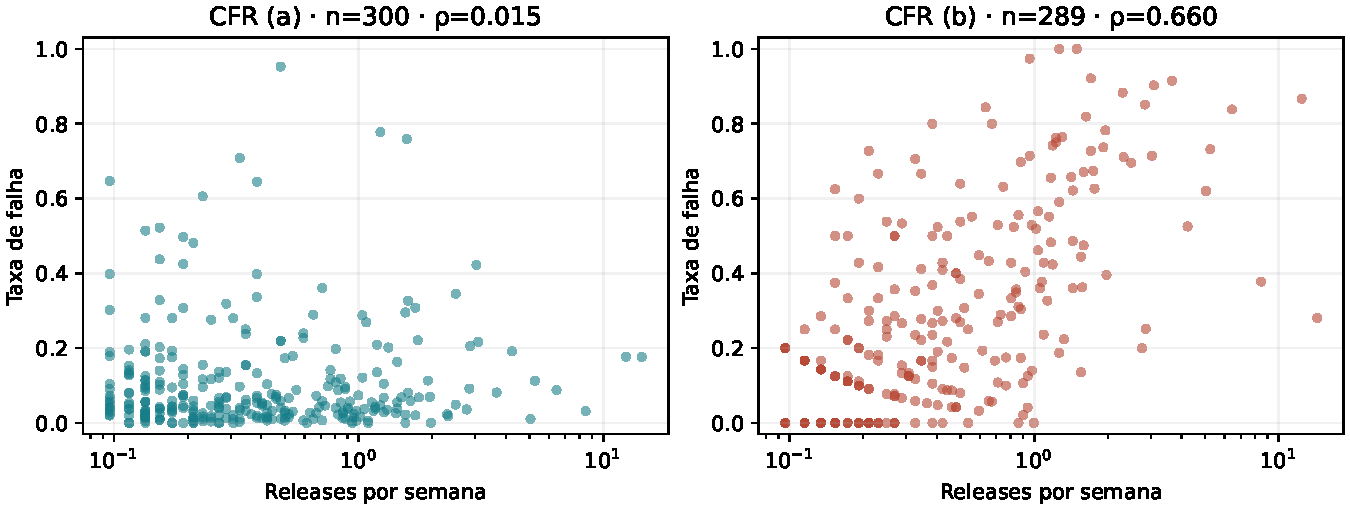
\includegraphics[width=\textwidth]{../../results/s03_b/rq05_dispersao.pdf}
\caption{RQ05: os mesmos projetos, mas proxies distintos de falha. Só a frequência
usa escala logarítmica; taxas zero são preservadas.}
\label{fig:rq05-final}
\end{figure}

\subsection{RQ06: fatores associados}

Seis dos 18 testes permanecem significativos após Holm (Tabela~\ref{tab:rq06-final}).
Contribuidores e linguagem associam-se aos lead times; contribuidores também à
recuperação, e tipo apenas à recuperação. Não há evidência após Holm para
frequência ou CFR em nenhum fator. H6 é parcial: linguagem não é menos relevante
que tipo, e associações não demonstram capacidade causal das comunidades.
Testes globais não identificam pares específicos; não executamos post-hoc.
Os 18 resultados e os tamanhos de cada grupo permanecem nos CSVs suplementares.

\begin{table}[htbp]
\centering\footnotesize
\caption{RQ06: testes que sobrevivem a Holm; todos são Kruskal--Wallis nesta amostra.}
\label{tab:rq06-final}
% Gerado por analises.sprint3_b
\begin{tabular}{llrrr}
\hline
Fator & Métrica & $n$ & $p$ Holm & $\varepsilon^2$ / $\delta$ \\
\hline
Tipo do projeto & Recuperação & 278 & 0,0347 & 0,051 \\
Contribuidores (quartis) & Lead time (a) & 300 & $8,10\times 10^{-7}$ & 0,124 \\
Contribuidores (quartis) & Lead time (b) & 300 & $6,11\times 10^{-9}$ & 0,157 \\
Contribuidores (quartis) & Recuperação & 278 & 0,0092 & 0,062 \\
Linguagem & Lead time (a) & 300 & 0,0002 & 0,124 \\
Linguagem & Lead time (b) & 300 & 0,0199 & 0,084 \\
\hline
\end{tabular}

\end{table}

\subsection{RQ07: sensibilidade das classificações}

C1 é reproduzida exatamente antes das comparações. C1 possui 278 classificações;
C2/C3, 269. Nove projetos perdem classificação porque trocar CI por CFR~(b)
introduz uma métrica ausente; isso não é contado como troca de categoria.
A Tabela~\ref{tab:rq07-final} separa populações por par e comum às três
(coincidentes nesta amostra). As matrizes da Figura~\ref{fig:rq07-final} mostram
inclusive os zeros e a direção das trocas.

\begin{table}[htbp]
\centering\footnotesize
\caption{RQ07: mudanças de categoria e Cohen linear; sem par = excluídos do cálculo.}
\label{tab:rq07-final}
% Gerado por analises.sprint3_c.
\begin{tabular}{llrrrrr}
\hline
Par & População & $n$ & Mudaram & \% & $\kappa_w$ & Sem par \\
\hline
C1--C2 & Por par & 269 & 106 & 39,4 & 0,455 & 31 \\
C1--C2 & Comum às três & 269 & 106 & 39,4 & 0,455 & 31 \\
C1--C3 & Por par & 269 & 108 & 40,1 & 0,437 & 31 \\
C1--C3 & Comum às três & 269 & 108 & 40,1 & 0,437 & 31 \\
C2--C3 & Por par & 269 & 12 & 4,5 & 0,931 & 31 \\
C2--C3 & Comum às três & 269 & 12 & 4,5 & 0,931 & 31 \\
\hline
\end{tabular}

\end{table}

\begin{figure}[htbp]
\centering
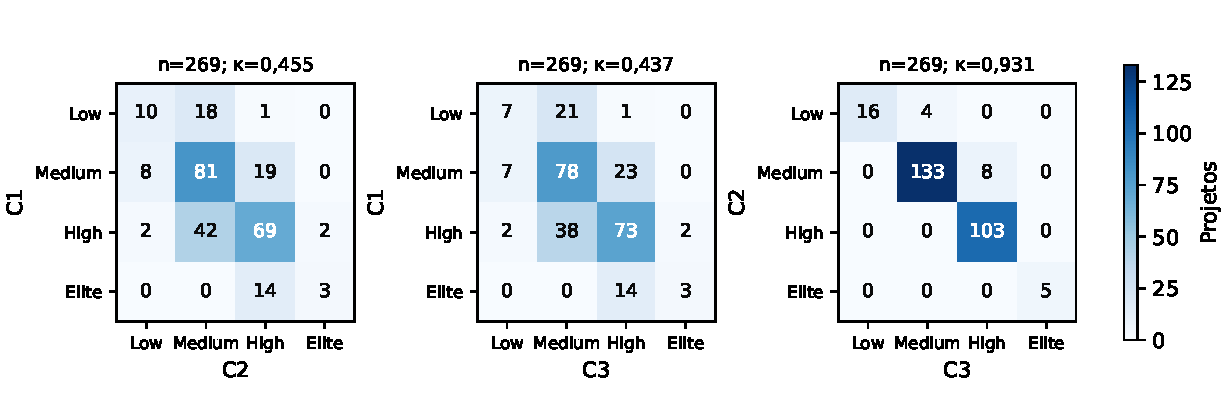
\includegraphics[width=\textwidth]{../../results/s03_c/rq07_transicoes.pdf}
\caption{Categorias gerais, de Low a Elite. Linha: combinação de origem;
coluna: destino. Ausências não entram como categoria.}
\label{fig:rq07-final}
\end{figure}

C1--C2 muda \labCCUmCDoisMudou\% dos \labCCUmCDoisN\ projetos
($\kappa_w=\labCCUmCDoisKappa$); C1--C3, \labCCUmCTresMudou\%
($\kappa_w=\labCCUmCTresKappa$). C2--C3 muda só \labCCDoisCTresMudou\%
($\kappa_w=\labCCDoisCTresKappa$). H7 é parcialmente sustentada: há concordância
moderada a alta, mas trocar conjuntamente lead time e CFR reclassifica cerca de
quatro em dez projetos. Essas comparações não isolam o efeito de cada mudança.

As conclusões de RQ01--RQ04 mantêm baixa frequência, lead time de vários dias,
diferença entre proxies de falha e recuperação tipicamente curta. A recuperação
é invariável por construção nas três combinações, não uma nova confirmação empírica.
Na RQ05, trocar a fonte da frequência mantém CI sem evidência após Holm e CFR~(b)
positivo ($\rho$ entre 0,599 e 0,660; $p$ ajustado 0,0012 na família de seis).
Na RQ06 ampliada, nenhuma frequência se associa aos fatores após Holm.
As associações de contribuidores/linguagem aos lead times e de contribuidores à
recuperação persistem; tipo--recuperação deixa de atingir 5\% na família de 24.
Isso mostra sensibilidade à multiplicidade, sem apagar o teste original de H6.

\subsection{RQ08 bônus: rework rate}

Escolhemos uma opção: releases principais corretivas divididas pelo total de
principais na janela, usando a v3 e a disponibilidade da RQ03~(b). Não censuramos
os últimos sete dias, pois não é preciso observar uma release futura para contar
a própria corretiva. A mediana é \labCReworkMediana\%, com \labCReworkN\ projetos
e \labCReworkAusentes\ ausentes. Nos mesmos projetos, rework supera CFR~(b) em
\labCReworkMaior\ casos; diferença pareada mediana de \labCReworkDifMediana\ pontos
percentuais. Não é a mesma medida: CFR conta as releases anteriores seguidas de
corretiva em sete dias. Uma corretiva pode marcar várias anteriores como falhas,
mas é contada uma vez em rework. Quatro releases em dias consecutivos, apenas a
última corretiva, dão 25\% de rework e 75\% de CFR, fora da fronteira censurada.

A regra herdada pode produzir negativos sem antecessora/commits. A sensibilidade
de evidência completa torna desconhecidas \labCReworkSemEvidencia\ de
\labCReworkTotal\ releases e deixa \labCReworkConservadorN\ projetos avaliáveis,
com mediana \labCReworkConservadorMediana\%. Tratar todas as desconhecidas como
negativas/positivas delimita a proporção agregada por release entre
\labCReworkLimInf\% e \labCReworkLimSup\%. Não são intervalos de confiança nem
medianas por projeto, e não incluem erros da heurística. O DORA observa implantações
não planejadas por incidentes em produção~\cite{doraMetricas}; nosso proxy de releases
corretivas não comprova essas condições.
